% Package
\documentclass[11pt]{article}

\usepackage{amsmath}
\usepackage{cite}
\usepackage{graphicx}
\usepackage[utf8]{inputenc}
\usepackage[T1]{fontenc}
\usepackage{lmodern}
\usepackage[ngerman]{babel}
\usepackage{hyphenat}
\usepackage{placeins}
\usepackage{subfig}

\title{ADP Aufgabe 2: Naives und Komplexes Sortieren}
\author{Team 1\\Hugo Protsch, Justin Hoffmann}

% Document
\begin{document}

    \maketitle

    \tableofcontents

    \newpage


    \section{Formales}\label{sec:Formales}

    \paragraph*{Aufgabenaufteilung}\mbox{}\\
    Der Entwurf für Insertion Sort wurde zusammen entwickelt.\\
    Der Entwurf für Quick Sort wurde von Hugo Protsch entwickelt.\\
    Der Entwurf für Heap Sort wurde von Justin Hoffmann entwickelt.

    \paragraph*{Quellenangaben}\mbox{}\\
    Es wurden lediglich Vorlesungsmaterialien verwendet.

    \paragraph*{Bearbeitungszeitraum}\mbox{}\\
    Der gesamte Arbeitsaufwand für den Entwurf belief sich auf x Stunden%TODO
    und teilt sich wie folgt auf:
    \begin{itemize}
        \setlength\itemsep{0em}
        \item Entwurf: ca. 18 Stunden
        \item Implementation: ca. 6 Stunden %TODO Justin
        \item Laufzeitmessung und Analyse: ca. 9 Stunden
    \end{itemize}

    \paragraph*{Aktueller Stand}\mbox{}\\
    Der Entwurf steht zur Implementation zur Verfugung.

    \paragraph*{Änderungen des Entwurfes}
    \begin{itemize}
        \setlength\itemsep{0em}
        \item Insertion Sort: Formulierung im Graph geändert
        \item Quicksort: Pivot-Element Wahl hinzugefügt
        \item Quicksort: Verzweigung zu Insertion Sort hinzugefügt
        \item Das Dokument wurde leicht umstrukturiert (Sektion-Hierarchy)
    \end{itemize}


    \section{Entwurf}\label{sec:entwurf}
    \subsection{Insertion Sort}\label{subsec:insertion-sort}

\paragraph{Algorithmus}\label{subsec:Ialgorithmus}
Siehe Abbildung~\ref{fig:insertionS}.
Bei Insertion Sort wird eine Liste durch das Einfügen von Elementen aus
einem unsortierten Bereich (zunächst die komplette Liste) in einen sortieren
Bereich (zunächst leer, <N1>) sortiert.

Bei dem Einfügen eines Elements E in den sortierten Bereich muss dabei
jeweils der Bereich bis zu dem Element durchlaufen werden, hinter das das
Element E eingefügt werden muss (Siehe \frqq Insert into sorted list\flqq
Subgraph).

Somit wird der sortierte Bereich mit jeder Iteration um 1 erhöht <E1>.
Sobald der sortierte Bereich alle Elemente enthält, wird die Liste
zurückgegeben.
Bei der Implementation des Algorithmus auf einfach verkettete Listen
kann der sortierte und unsortierte Bereich getrennt werden.


\begin{figure}[hbt]
    \caption{Insertion Sort}
    \centering
    \includegraphics[width = 8cm]{insertionS}\label{fig:insertionS}
\end{figure}
\FloatBarrier

\paragraph{Laufzeit}\label{subsubsec:ilaufzeit}
Die erwartete Laufzeit beträgt \(O(n^2)\), da bei jeder Iteration das
einzufügende Element mit allen noch nicht sortierten Elementen verglichen
wird.
Im Fall einer bereits sortierten Liste tritt der Best-Case ein.
Hierbei müssen nur \(n\) Vergleiche durchgeführt werden.
Somit beträgt die Laufzeit \(\Theta(n)\).

Bei der Laufzeitmessung überprüfen wir, ob der gemessene Zusammenhang mit
dem erwarteten übereinstimmt.
Dafür verwenden wir für den Best-Case zufällige Listen, im Worst-Case
bereits sortierte Listen.


\subsection{Quick Sort}\label{subsec:quick-sort}

\paragraph{Algorithmus}\label{subsec:Qalgorithmus}
Siehe Abbildung~\ref{fig:qsort}.
Bei Quick Sort wird zunächst willkürlich ein Pivot-Element aus der Liste
ausgewählt.

Anschließend wird die Liste in zwei Teile aufgeteilt: Die Liste L erhält
alle Elemente, die kleiner als das Pivot-Element sind, die Liste R alle
Elemente, die größer als das Pivot-Element sind.
Dafür wird die Liste elementweise durchlaufen und jedes Element mit dem
Pivot-Element verglichen.
Die Reihenfolge der Elemente in den Listen spielt keine Rolle.
Das Pivot-Element selber kommt nicht in den Listen vor.

Da alle Elemente, die kleiner als das Pivot-Element sind und alle Elemente,
die größer als das Pivot-Element sind nun getrennt vorliegen, ist die
Position des Pivots eindeutig als 'zwischen den Listen L und R' bestimmt.
Somit kann der Algorithmus rekursiv auf die jeweiligen Listen erneut
angewandt werden.

Das Pivot-Element wird an die Liste R vorangestellt.
Die Liste L wird der Liste R, inklusive Pivot, vorangestellt.
Die Liste ist nun sortiert.\\

\begin{figure}[hbt]
    \caption{Quicksort}
    \centering
    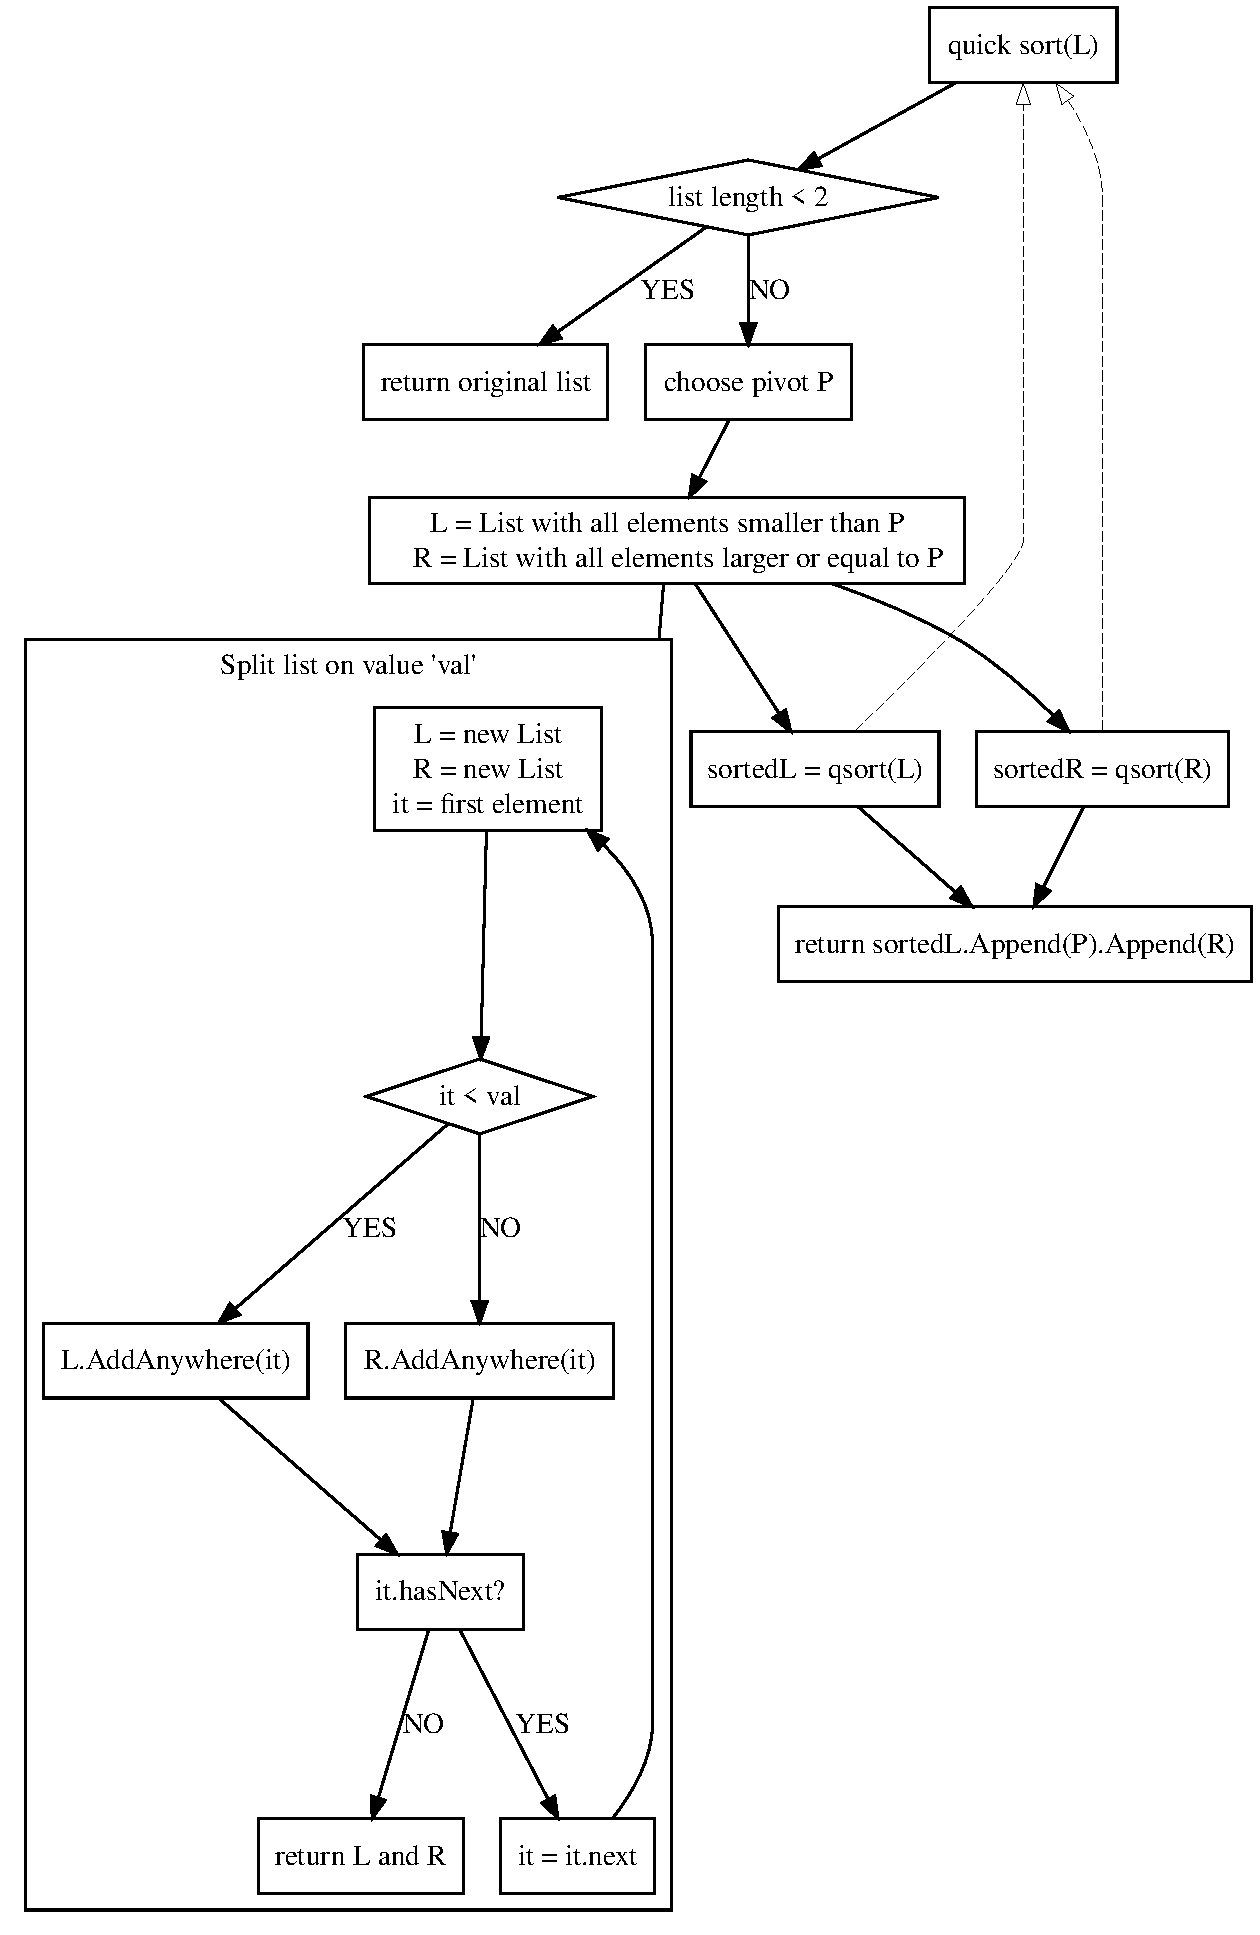
\includegraphics[width = 8cm]{qsort.pdf}\label{fig:qsort}
\end{figure}

Für die Wahl des Pivot-Elementes werden insgesamt 5 Methoden implementiert:
\begin{itemize}
    \item left -- wählt das erste Elemente der Liste
    \item middle -- wählt das mittlere Element der Liste
    \item right -- wählt das letzte Element der Liste
    \item median -- wählt den Median der drei obigen Werte
    \item random -- wählt ein zufällig ausgewähltes Element der Liste
\end{itemize}

Des Weiteren soll bei der Implementation des Algorithmus ab einem
Schwellenwert auf Insertion Sort umgeschaltet werden.
Dafür wird zu Beginn die Länge der Liste abgefragt, falls diese unter dem
übergebenem Schwellenwert liegt, wird restliche Liste stattdessen
mithilfe von Insertion Sort sortiert.

\FloatBarrier

\paragraph{Laufzeit}\label{subsec:Qlaufzeit}

Die Laufzeit beträgt im Best-Case \(\Omega (n \cdot \log(n))\), da bei
gut gewähltem Pivot-Elementen die Anzahl an Vergleichen mit jedem
Rekursionsschritt halbiert wird, wobei die Teillisten trotzdem durchlaufen
werden müssen.
Wenn das Pivot-Element bei jeder Iteration schlecht gewählt ist (kleinstes
oder größtes Element in der List), beträgt die Laufzeit \(O(n^2)\), da
jeweils eine Partition die Größe 1 hat und die Anzahl an Vergleichen
somit nicht reduziert wird.

Bei der Laufzeitmessung testen wir, ob die Komplexität des implementierten
Algorithmus mit der erwarteten übereinstimmt.
Um den Worst-Case zu überprüfen, nutzen wir bereits sortierte Listen und
wählen das letzte bzw. erste Element als Pivot-Element.
Für den Best-Case nutzten wir zufällig generierte Listen.\\

Wir ermitteln des Weiteren die Elementanzahl, ab der Quicksort schneller
als Insertion Sort ist und wie sich die unterschiedlich Methoden, das
Pivot-Element auszuwählen, auf die Laufzeit auswirken.

Außerdem wird die Implementation mit Erlang List Comprehension der
Eigenen gegenübergestellt.
Wir erwarten bei der List Comprehension eine leicht langsamere Laufzeit als
bei der eigenen Implementierung, da bei der List Comprehension die Liste
zwei Mal durchlaufen wird:
Das erste Mal um alle Elemente, die größer -- das zweite Mal
um alle Elemente, die kleiner als das Pivot-Element sind, zu filtern.
Bei der eigenen Implementation wird die Liste lediglich einmal
durchlaufen.
Hierbei ist es interessant zu sehen, inwiefern sich die Anzahl an
Durchläufen durch die Liste in der Laufzeit wieder spiegelt.


\subsection{Heap Sort}\label{subsec:heap-sort}

\paragraph{Algorithmus}\label{subsubsec:halgorithmus}

\subparagraph{Allgemeiner Aufbau}
Betrachte Abbildung~\ref{fig:hsortentwurf}.
Im Allgemeinen besteht Heap Sort im Wesentlichen aus zwei Teilen:
Dem Bauen eines Max-Heaps aus der zu sortierenden Liste und dem
eigentlichen Sortieren mithilfe dieses Heaps.
Der sogenannte Max-Heap ist eine binäre Baum-Datenstruktur, in der jeder
Kindwert kleiner dem Elternwert ist, die entscheidende Eigenschaft für
den Heap-Sort.

Strukturell haben wir einen "Divide and Conquer"-Ansatz gewählt und den
Algorithmus in mehrere Subroutinen unterteilt.

\subparagraph{Bauen des Max-Heaps}
Der Bau-Algorithmus des Max-Heaps beginnt mit dem Inkrementieren der Heap-Size, da ein neues Element eingesetzt wird.
Jedes nachfolgende Element wird unten eingefügt.
Der Baum wird von links nach rechts und top-down aufgebaut.
Jeder Funktionsdurchlauf berechnet den Einsetz-Pfad im Heap.
Wir vergleichen den derzeitigen Knoten mit unserem temporären Laufwert.
Ist dieser Laufwert größer als der derzeitige Knoten, werden beide Werte vertauscht, sprich der Laufwert wird in den derzeitigen Knoten eingesetzt und der (nun ehemalige) derzeitige Knoten wird zum temporären Laufwert.
So "sickert" jeder Wert aus der Liste and die richtige Position im Max-Heap, bis der korrekte Pfad abgelaufen worden ist.

In Abbildung~\ref{fig:buildMaxHeap} spiegelt sich dieser Absteig-Vorgang
in der unteren Schleife wieder.

\subparagraph{Heapify}
In Heapify (siehe Abbildung~\ref{fig:heapify}) machen wir uns die
Tatsache zunutze, dass eigentlich ein
Max-Heap vorliegt und sich nur ein einziges Element an der falschen
Stelle befindet.
Dieses Element wird, falls nötig, zu einer passenden Position nach unten
"durchsickern".

Zunächst wird überprüft, ob das beide Kinder der derzeitigen Postion im Baum (beim ersten Durchlauf root) leer sind, wir also einen Knoten ohne Kinder vorliegen haben.
Ist dies der Fall sind wir am Ende des Baumes und geben den Heap zurueck.
Ist dies nicht der Fall, kann es sein, dass nur das rechte Kind leer ist, was ebenfalls ueberprueft wird.
Dies bedeutet, dass das linke Kind das letzte Element im Heap ist.
Ein letzter Vergleich mit dem linken Kind (und ein letzter Tausche falls noetig) und der Baum wird zurueckgegeben.
Das eigentliche "Durchsickern" des Lauf-Elements passiert nach diesen beiden Abfragen.
Bei jeder Position wird zunaechst ueberprueft, ob das Lauf-Element groesser als beide Kinder ist.
Ist dies der Fall ist das Element an die richtige Stelle durchgesickert.
Ist dies jedoch nicht der Fall, tauscht das Element mit dem jeweils groesseren Kind die Position und wandert so nach unten.

So wird der Heap für die weitere Sortierung "heapified".

\subparagraph{Sortierung}
Auf das Umwandeln der Liste in einen Max-Heap wurde bereits eingegangen.
Der erstellte Max-Heap wird dann zum Sortieren benutzt.
Wie oben bereits erwähnt ist die bestimmende Eigenschaft eines Max-Heaps
der ausschlaggebende Aspekt dieses Sortier-Algorithmus.
Wir fügen also das Wurzelelement des Heaps in die Output-Liste ein.
Dieses Element gilt nun als sortiert (alle Elemente müssen vorne angefügt
werden).
Nun wird das letzte Element des Heaps mit der Wurzel getauscht und die
ehemalige Wurzel entfernt.
Die Struktur des Max-Heaps wird, wie oben beschrieben, durch Heapify
wieder hergestellt.
Dieser Vorgang wiederholt sich nachfolgend mit dem jeweils reduzierten
Max-Heap, bis keine Elemente mehr im Heap vorhanden sind.
Abschließend kann eine vollständige sortierte Liste zurückgegeben werden.

\begin{figure}[hbt]
    \caption{Heap Sort}
    \centering
    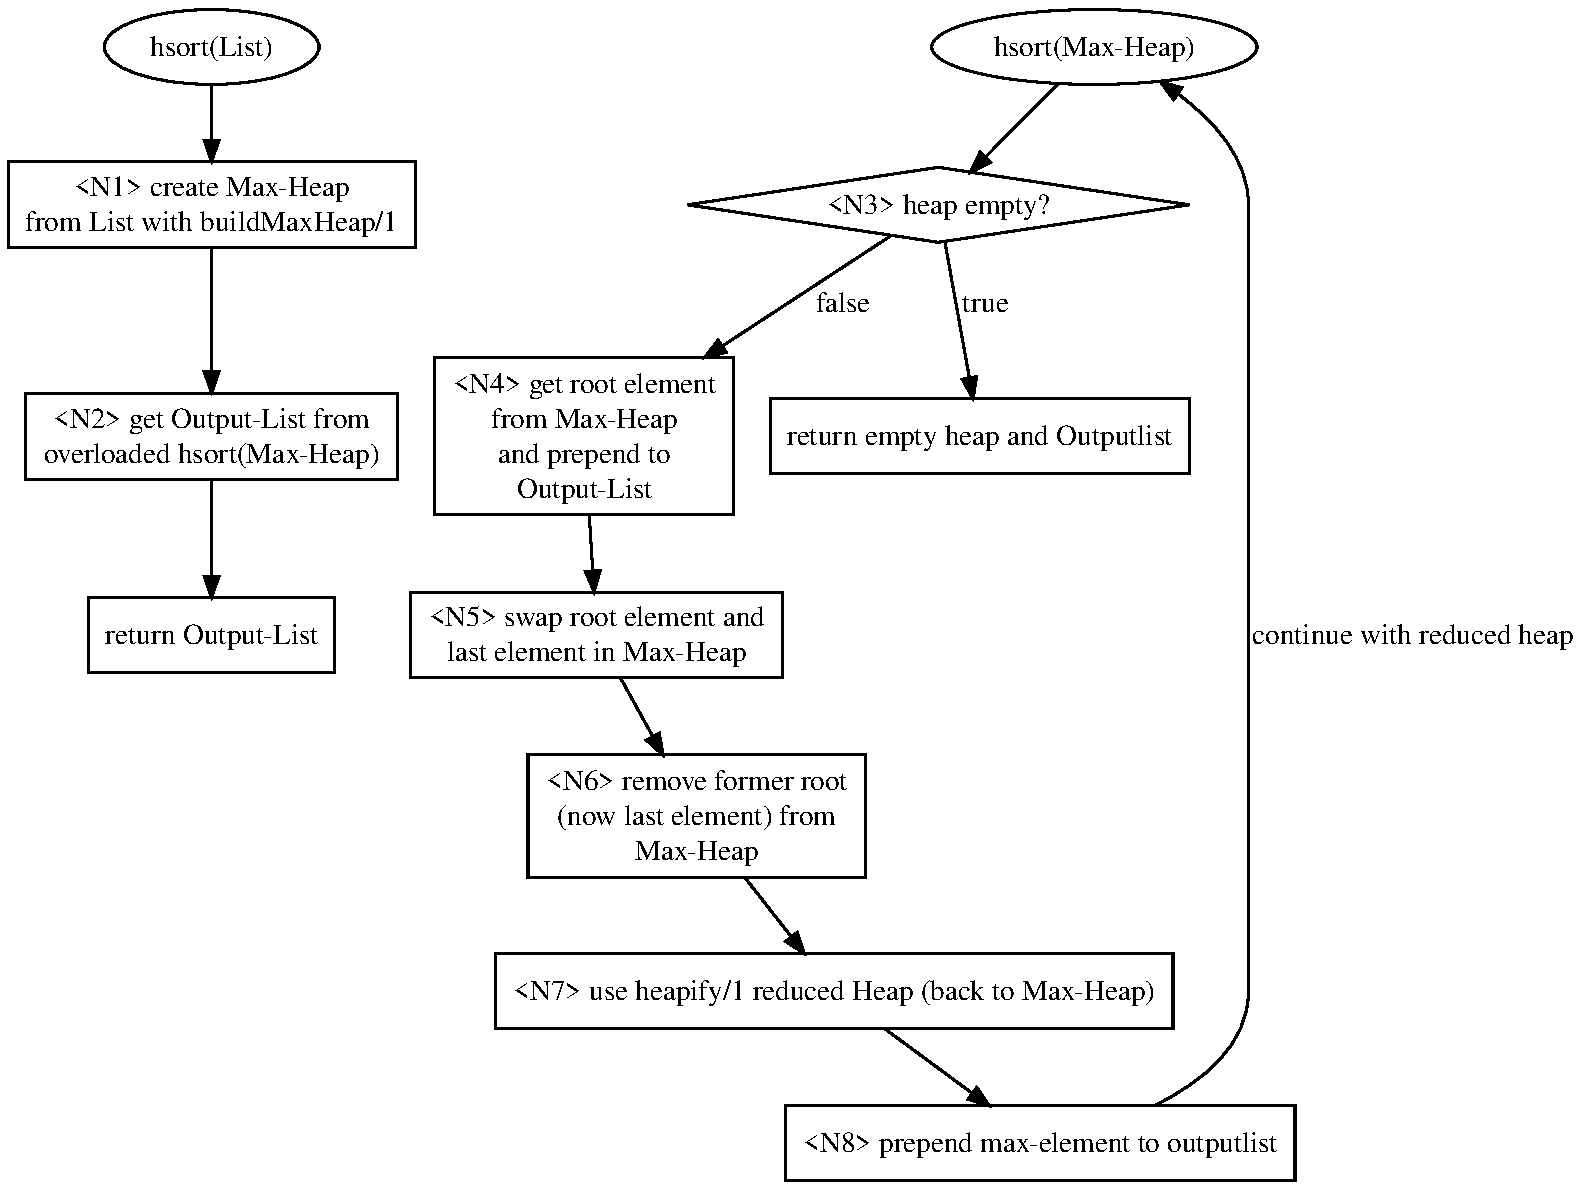
\includegraphics[width = 11cm]{hsort.pdf}\label{fig:hsortentwurf}
\end{figure}

\begin{figure}[hbp]
    \caption{Heapify}
    \centering
    \makebox[\textwidth][c]{
    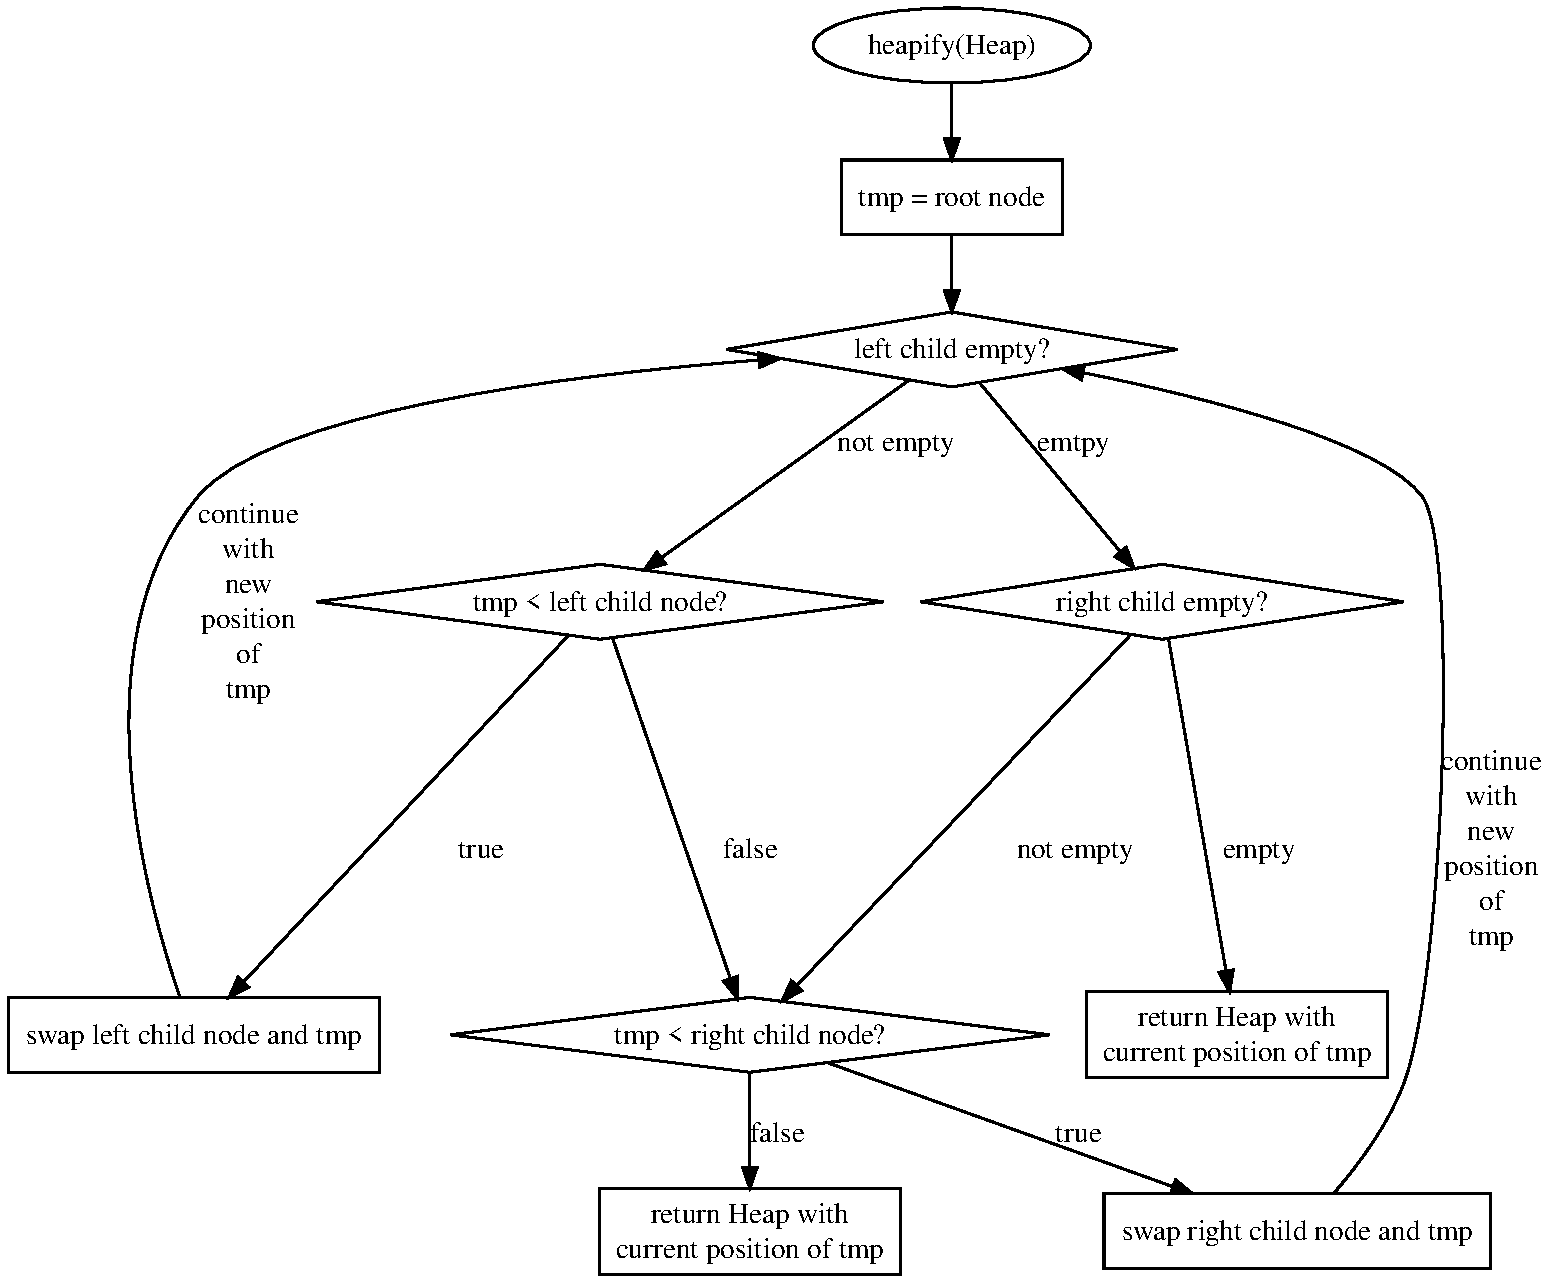
\includegraphics[width = 1.35\textwidth]{heapify.pdf}\label{fig:heapify}}

\end{figure}

\begin{figure}[hbtp]
    \caption{Build Max-Heap}
    \centering
    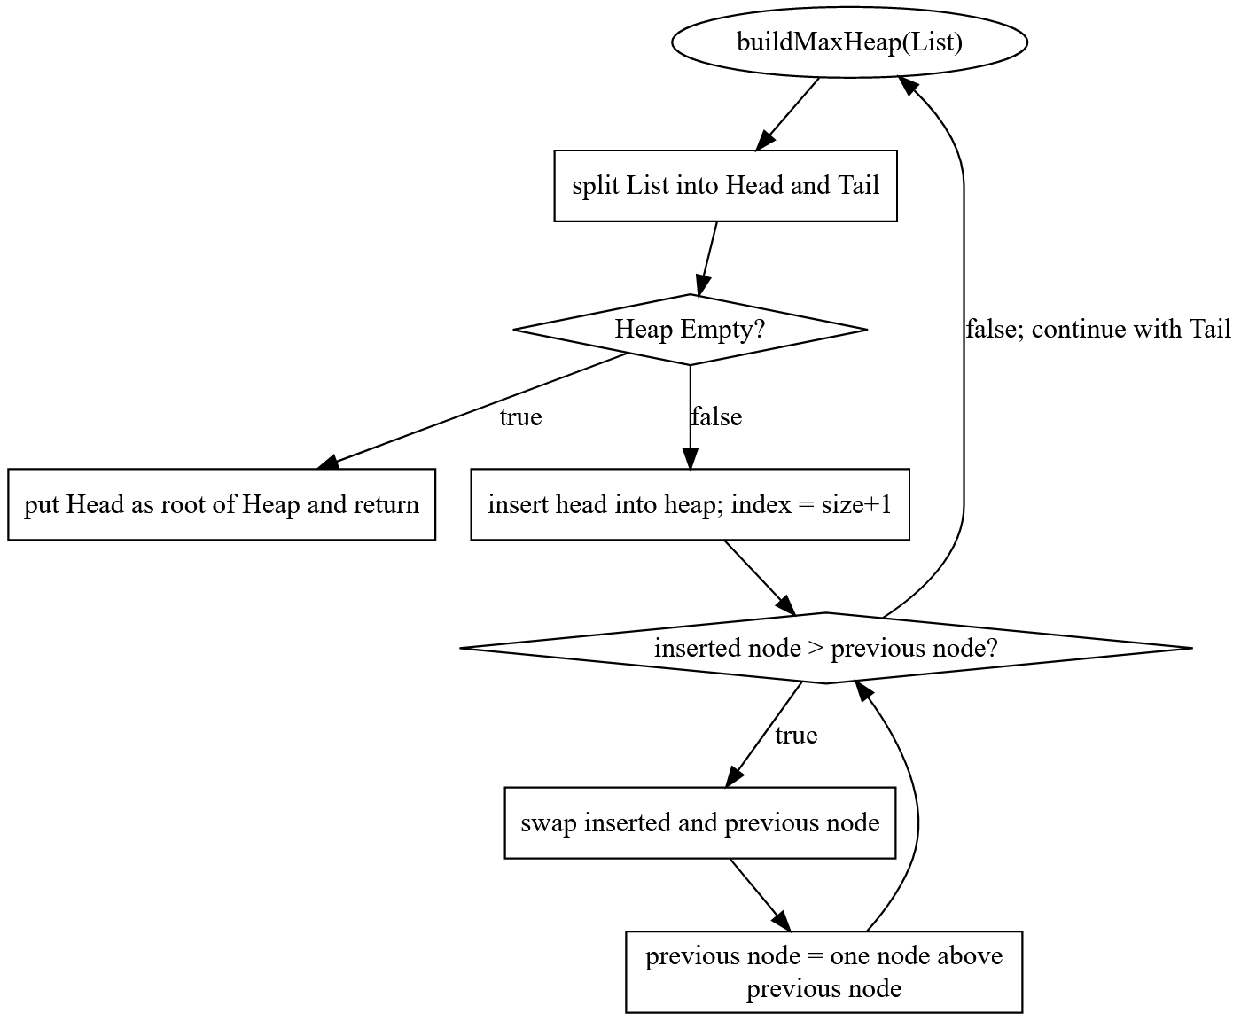
\includegraphics[width = 10cm]{buildMaxHeap.pdf}\label{fig:buildMaxHeap}
\end{figure}

\paragraph{Laufzeit}\label{subsec:Hlaufzeit}
Die Laufzeit beträgt im Worst-Case \(O(n\cdot log\ n)\). Dieser tritt
ein, wenn eine bereits weitgehend vorsortierte Liste vorliegt, da die
Liste beim Heap-Aufbau gewissermaßen invertiert wird und somit viele
Vergleiche pro Element erforderlich sind.
Wünschenswert wäre demnach eine invertiert-sortierte Liste, wodurch die
Anzahl der Vergleiche auf 1 pro Element minimiert ist.
Es gilt mit den Laufzeittests herauszufinden, ob unsere
Komplexitäts--Annahmen realistisch sind.
Um Heap-Sort hinreichend zu testen, binden wir den Algorithmus erweiternd
in den Quick-Sort-Test mit ein und stellen beide gegenüber.
Diese drei Fälle werden untersucht und verglichen:
\begin{samepage}
    \begin{itemize}
        \item Vorsortierte Liste
        \item Invertiert sortierte Liste
        \item Zufällig generierte Liste
    \end{itemize}
Wir erwarten, dass Heapsort nur dann schneller ist als Quicksort, wenn die fuer Quicksort unguenstigsten Bedingungen bestehen.
\end{samepage}
\FloatBarrier


    \newpage

    \section{Laufzeitmessung}\label{sec:laufzeitmessung}
    \subsection{Insertion Sort}\label{subsec:insertion-sort-laufzeit}

\subsection{Quick Sort}\label{subsec:quick-sort-laufzeit}

\subsubsection{Pivot Methoden}

\paragraph{Erste Implementation}
Bei der ersten Implementation vom Quicksort Algorithmus ist bei der
Verwendung der Pivot-Methoden \(right\) und \(median\)  eine deutlich längere
Laufzeit aufgefallen (siehe Abbildung~\ref{fig:qsort-first-impl}).
Gleichzeit ist die Laufzeit von der \(middle\) Pivot Methode besser, obwohl
die Erwartung dieser schlechter ist:
Diese muss eineinhalb mal -- einmal zum finden der Länge \(l\) komplett, danach
bis zum \(l/2\) Element -- durchlaufen werden.
Die Pivot Methode \(right\) muss nur einmal bis zum Ende der Liste laufen.

\begin{figure}[hbt]
    \caption{Vergleich der Pivot Methoden 1}
    \centering
    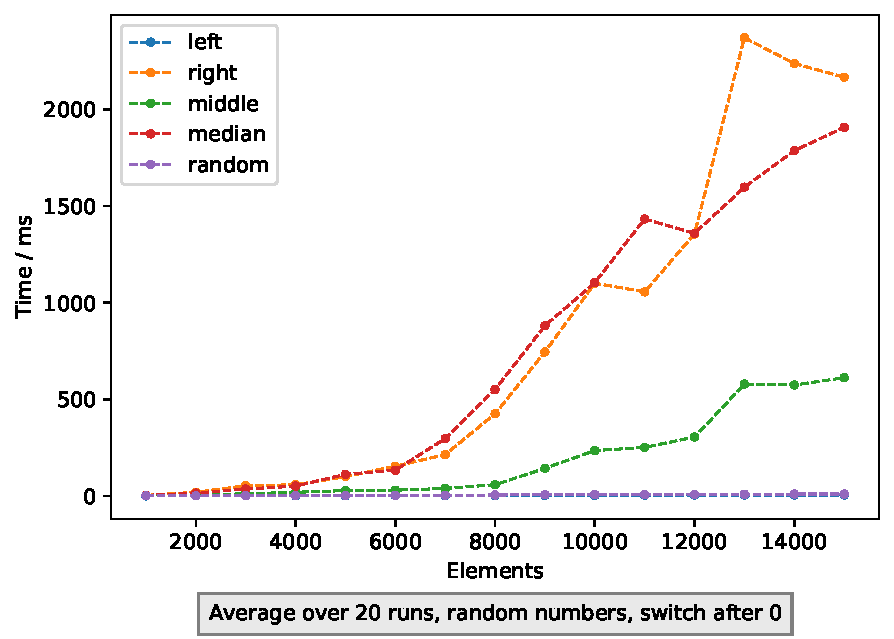
\includegraphics[width = 8cm]
    {../out/pivotMethods_Implementation1.pdf}\label{fig:qsort-first-impl}
\end{figure}

Unsere erste Vermutung war, dass unsere Methoden, die in einem
Durchlauf die Länge und gleichzeitig dass Pivot-Element ermitteln dafür
verantwortlich sein könnten.
In der Methoden zum Finden des letzten Elementes, die auch von der median
Pivot Methode verwendet wird, benutzten wir Pattern Matching, um zwischen dem
Letzten und vorletztem Element zu unterscheiden.
Dabei muss allerdings jeweils vorausgeschaut werden, was die schlechte
Performance erklären könnte.

Somit die Vermutung, dass man die Performance verbessern kann, indem man
zunächst die Länge der Liste ermittelt und anschließend diese zum Finden des
n-ten Elements ein zweites mal durchläuft.

\paragraph{Zweite Implementation}

In der zweiten Implementation wurden die Ermittlung des Pivots und das Finden
der Länge der Liste getrennt.
Das letzte Elements wurde nun ermittelt, indem zunächst
die Länge \(l\) der Liste berechnet, anschließend mithilfe dieser zum
\(l-1\) -ten Element gelaufen wird.
\begin{figure}[hbt]
    \centering
    \caption{Zweite Implementation}
    \subfloat[median]{
    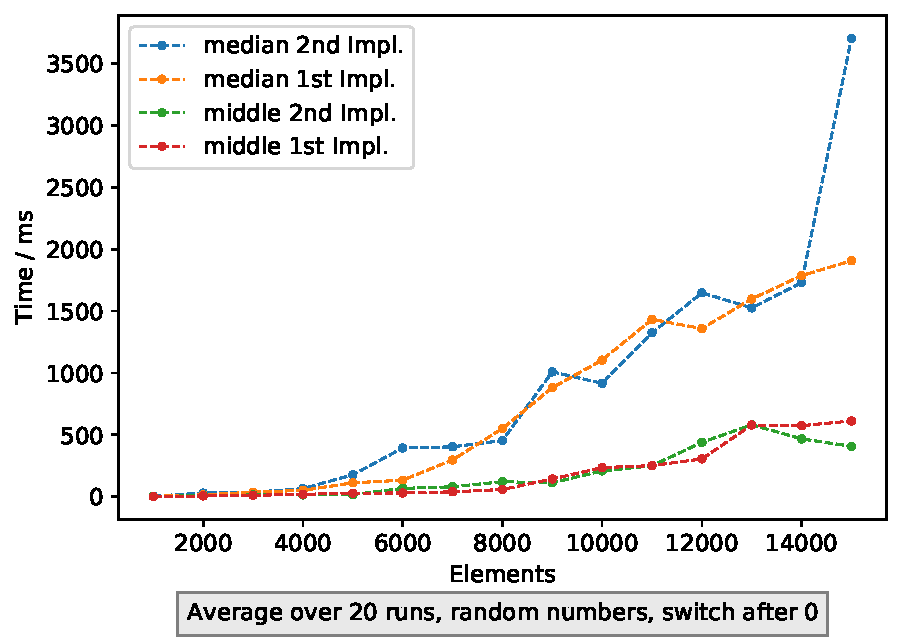
\includegraphics[width = 0.47\textwidth]
    {../out/pivotMethods_Implementation2b.pdf}\label{fig:qsort-impl2b} }
    \hfill
    \subfloat[right]{
    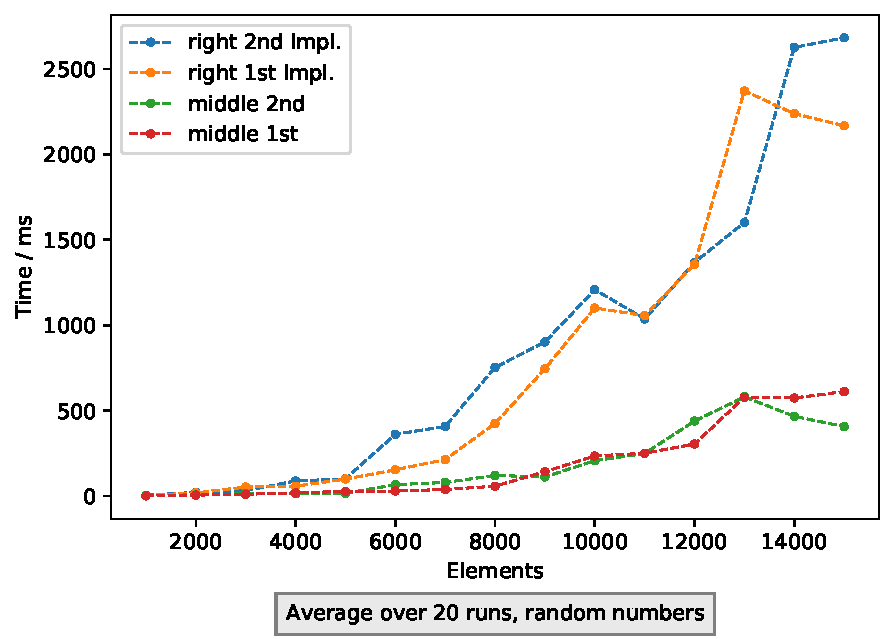
\includegraphics[width = 0.47\textwidth]
    {../out/pivotMethods_Implementation2a.pdf}\label{fig:qsort-impl2a} }
\end{figure}


In Abbildung~\ref{fig:qsort-impl2b} und~\ref{fig:qsort-impl2a} sind jeweils die
Ergebnisse der Laufzeitmessung der zweiten Implementation von \(median\) und
\(right\) zu sehen.
Damit systematische Unterschiede zwischen den beiden Kompilationen
ausgeschlossen sind, ist zusätzlich die gleiche Implementation, von \(middle\)
dargestellt.
Bei beiden überarbeiteten Implementationen ist keine Besserung der Laufzeit zu
erkennen, was darauf schließen lässt, dass das in der ersten Implementation
verwendete Pattern Matching nicht der Grund der schlechten Performance war.

\paragraph{Weitere Mögliche Ursachen}
Eine weitere Mögliche Ursache für die Ergebnisse ist der Fakt, das bei der
Methode zum finden des n-ten Elementes und des Restes
\textit{listGetNthAndRest()} die Erlang List Concatenation (\(++\)) verwendet
wird, und somit bei jedem Rekursionsschritt ein zusätzlicher Aufwand von
\(n\), wobei \(n\) die Anzahl der Elemente in der Subliste darstellt, hinzukommt.
Dies würde auch erklären, warum \textit{middle} eine bessere Laufzeit
aufweist, da dabei nur ein zusätzlicher Aufwand von \(n/2\) halbe dazukommt.

\paragraph{Dritte Implementation}
In der dritten Implementation wurde die List Concatenation ersetzt.

\begin{figure}[hbt]
    \centering
    \caption{Dritte Implementation}
    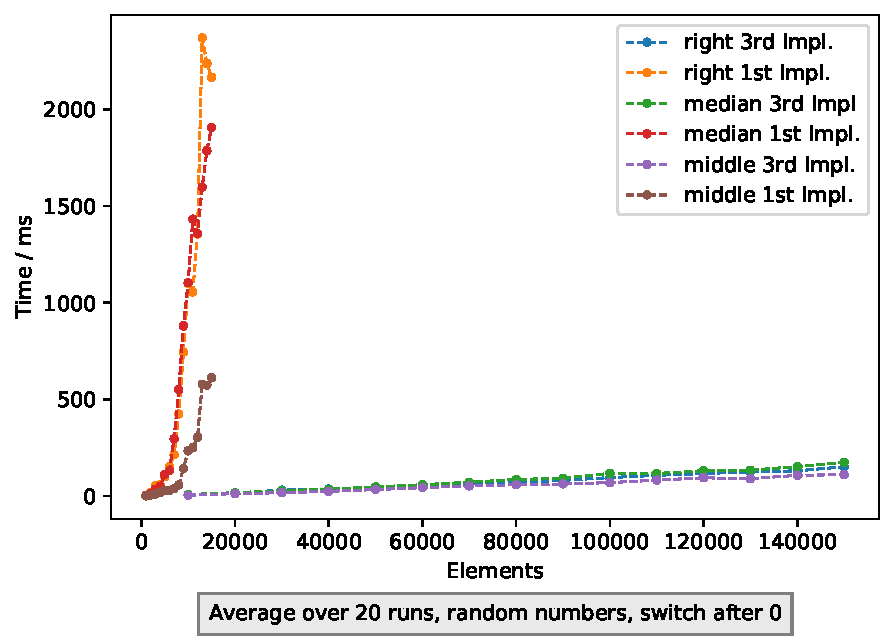
\includegraphics[width=8cm]
    {../out/pivotMethods_Implementation3.pdf}\label{fig:qsort-impl3}
\end{figure}

Wie in Abbildung~\ref{fig:qsort-impl3} zu sehen,
verbessert dies die Laufzeit dramatisch.
Die Laufzeit der Pivot Methode \textit{middle} hat sich auch verbessert, was
darauf zurückzuführen ist, dass diese ebenfalls die \textit{listGetNthAndRest
()} Methode verwendet.

\FloatBarrier

\subsubsection{Switch Number}
Bei der Implementation des Quicksort-Algorithmus wird ein Parameter
\textit{switchnumber} übergeben, welches den Schwellenwert angibt, ab wann
von Quicksort auf Insertion Sort umgeschaltet werden soll.
Zum Finden des optimalen Wertes dieses Parameters verwenden wir die Pivot
Methode \textit{left},

\subsection{Heap Sort}\label{subsec:heap-sort-laufzeit}



\end{document}
